% Software Development for Mobile Devices
\documentclass[11pt,english,numbers=endperiod,parskip=half]{scrartcl}

\usepackage{color}
\usepackage{graphicx}
\usepackage{minted}
\usepackage{fancyhdr}
\usepackage{pdflscape}
\usepackage{listings}
\usepackage{pifont}
\usepackage{pdfpages}
\usepackage{hyperref}
\usepackage{subcaption}

\newcommand{\cmark}{\ding{51}}

\pagestyle{fancy}

\rhead{Daniel Parker - 971328X}
\lhead{COS30017 - Software Development for Mobile Devices}

\title{Distinction Experience Report}
\subtitle{COS30017 - Software Development for Mobile Devices}
\author{Daniel Parker 971328X}

\date{\today}

\begin{document}
\maketitle
\thispagestyle{empty}

\section{Introduction}
  \centering
    \textbf{Perspective:} Design Communication Perspective

  \raggedright
    This document covers the experience of writing a non-trivial Android
    application from the perspective of communicating the design of the app,
    including class diagrams, navigation model and data model. It also covers
    limitations of API used in developing the program, as well as a short
    section on the experience of using RAPPT for prototyping during initial
    phases of development, and how that affected the continued development.

\section{Project Structure}
  The application is structured in part as per the Android standards, and also
  by how RAPPT has generated package structures and various utilities such as
  RESTful API client, error dialogs, listview and list adapters.

  \subsection{Resources}
    Resources are separated into;
    \begin{itemize}
      \item{anim}
      \item{drawable}
      \item{layou}
      \item{menu}
      \item{values}
    \end{itemize}
    There are different
    styles specified for API 21 than API 15+ due to the need to use the AppCompat
    themes and libraries for backwards compatibility of Material Design components,
    visual and navigation design patterns.

  \subsection{Source}
    Java source is separated as suggested by the output of RAPPT into the following
    packages;
    \begin{itemize}
      \item{activites}
      \item{adapters}
      \item{fragments}
      \item{interfaces}
      \item{model}
      \item{views}
    \end{itemize}
    Some application level source files are in the root of the java source to
    indicate their global importance to the project.

  \subsection{Libraries}
  Most libraries are included by gradle at compile time, however one library
  needed modifications, and has been packaged as a jar archive and added
  to the libs directory and as a gradle dependency.
\section{Program Structure}
  Much of the app is structured in the `predefined' manner which is mostly
  dictated by the Android libraries and framework. These structural aspects can
  mostly be observed in the class diagram, and are highlighted by the
  inheritance of one of the green coloured Android classes by one of the app's
  classes. Other important structural parts which aren't shown in the class
  diagram due to their complexity are;
  \begin{itemize}
      \item{
        Activities/Fragments which contain listviews in their layout will
        utilise one of the Adapter classes to map a Parcelable model to
        the correct View objects in the Activity.
      }
      \item{
        Activities instantiate Fragments and then use the FragmentManager
        and FragmentTransactions to manage what fragments are in view,
        how they are animated onto and off the screen, and whether they are
        placed onto the backstack.
      }
      \item{
        The TrendchattrApplication class contains a socket.io service which
        will notify all registered classes that implement the RoomListener
        interface that a new message has arrived. It also manages the shared
        preferences, sending of chat messages and contains the TrendchattrApi
        object which executes all the RESTful API calls.
      }
  \end{itemize}

  Data management and flow is particularly interesting for trendChattr in that
  it requires both RESTful API calls and instantaneous asynchronous chat
  communications. This is achieved by using a Node.js server which manages
  user and trend data in a Mongo database, and has a small part which manages
  the connecting and broadcasting of clients to socket.io rooms. The app connects
  to this server using the Retrofit library for REST requests (ie. Registration,
  Login, Chatroom list), and using the socket.io-client java library to respond
  to and emit socket.io events and enabling instant messenger chat communication.

  Additionally, upon logging in the server will require that all requests are
  accompanied by a security token which is generated and sent back as a response
  to the login request. Retrofit manages the inclusion of this token to all
  the relevant API calls by adding it to the HTTP header, and the server will
  ensure that the user is authenticated to perform the tasks that they try to.
  Tokens only become invalid if the user logs back in again, as the token will
  be regenerated and the old one lost.

  \textit{\textbf{NOTE: }The trending topics are sourced from Twitter and are
  hard-coded to be relevant to the Melbourne region. Due to the Twitter API
  limiting the frequency of requests to this endpoint, the Node.js server will
  update the trends itself using a cron job and always supply to the app trends
  relevant to the last 5 minutes.}
  \newpage
  \subsection{Class Diagram}
    \begin{figure}[H]
      \centering{
        \fbox{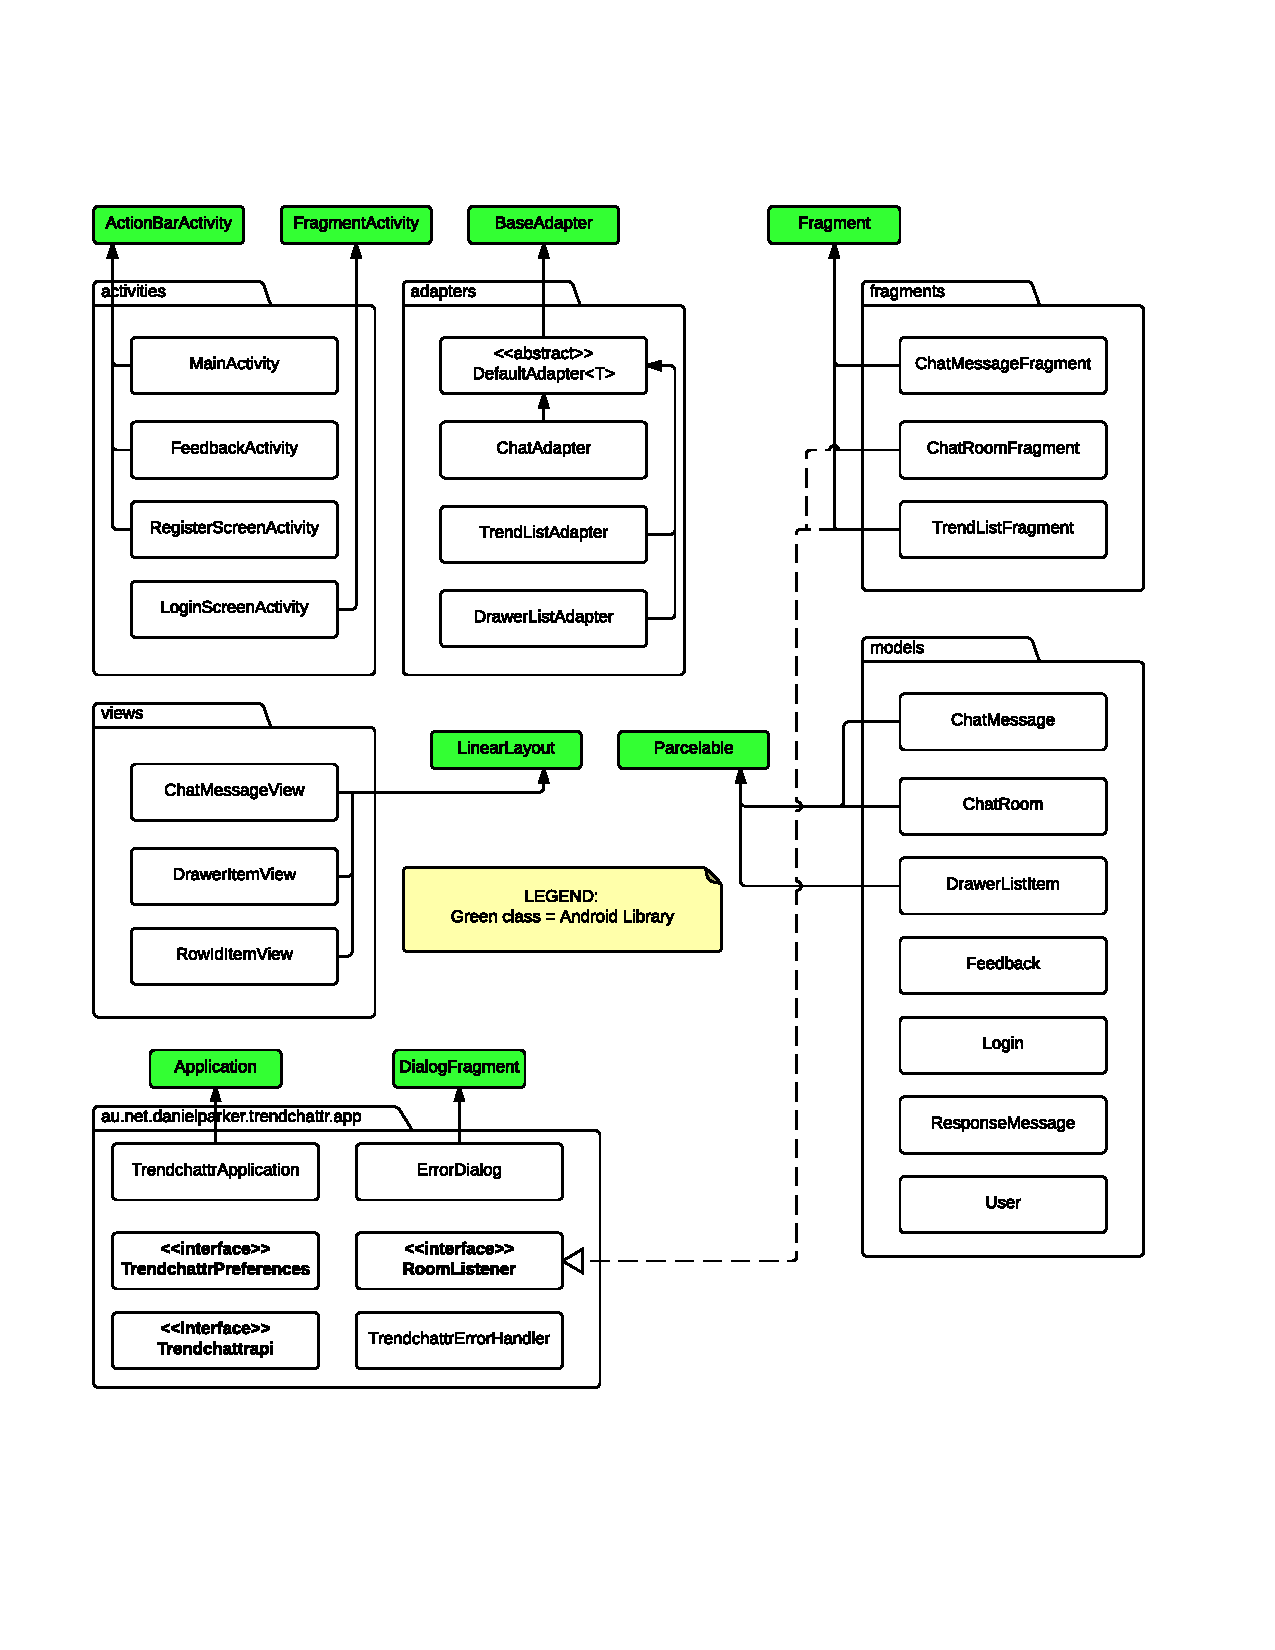
\includegraphics[width=\textwidth]{classes.pdf}}
      }
    \end{figure}
    %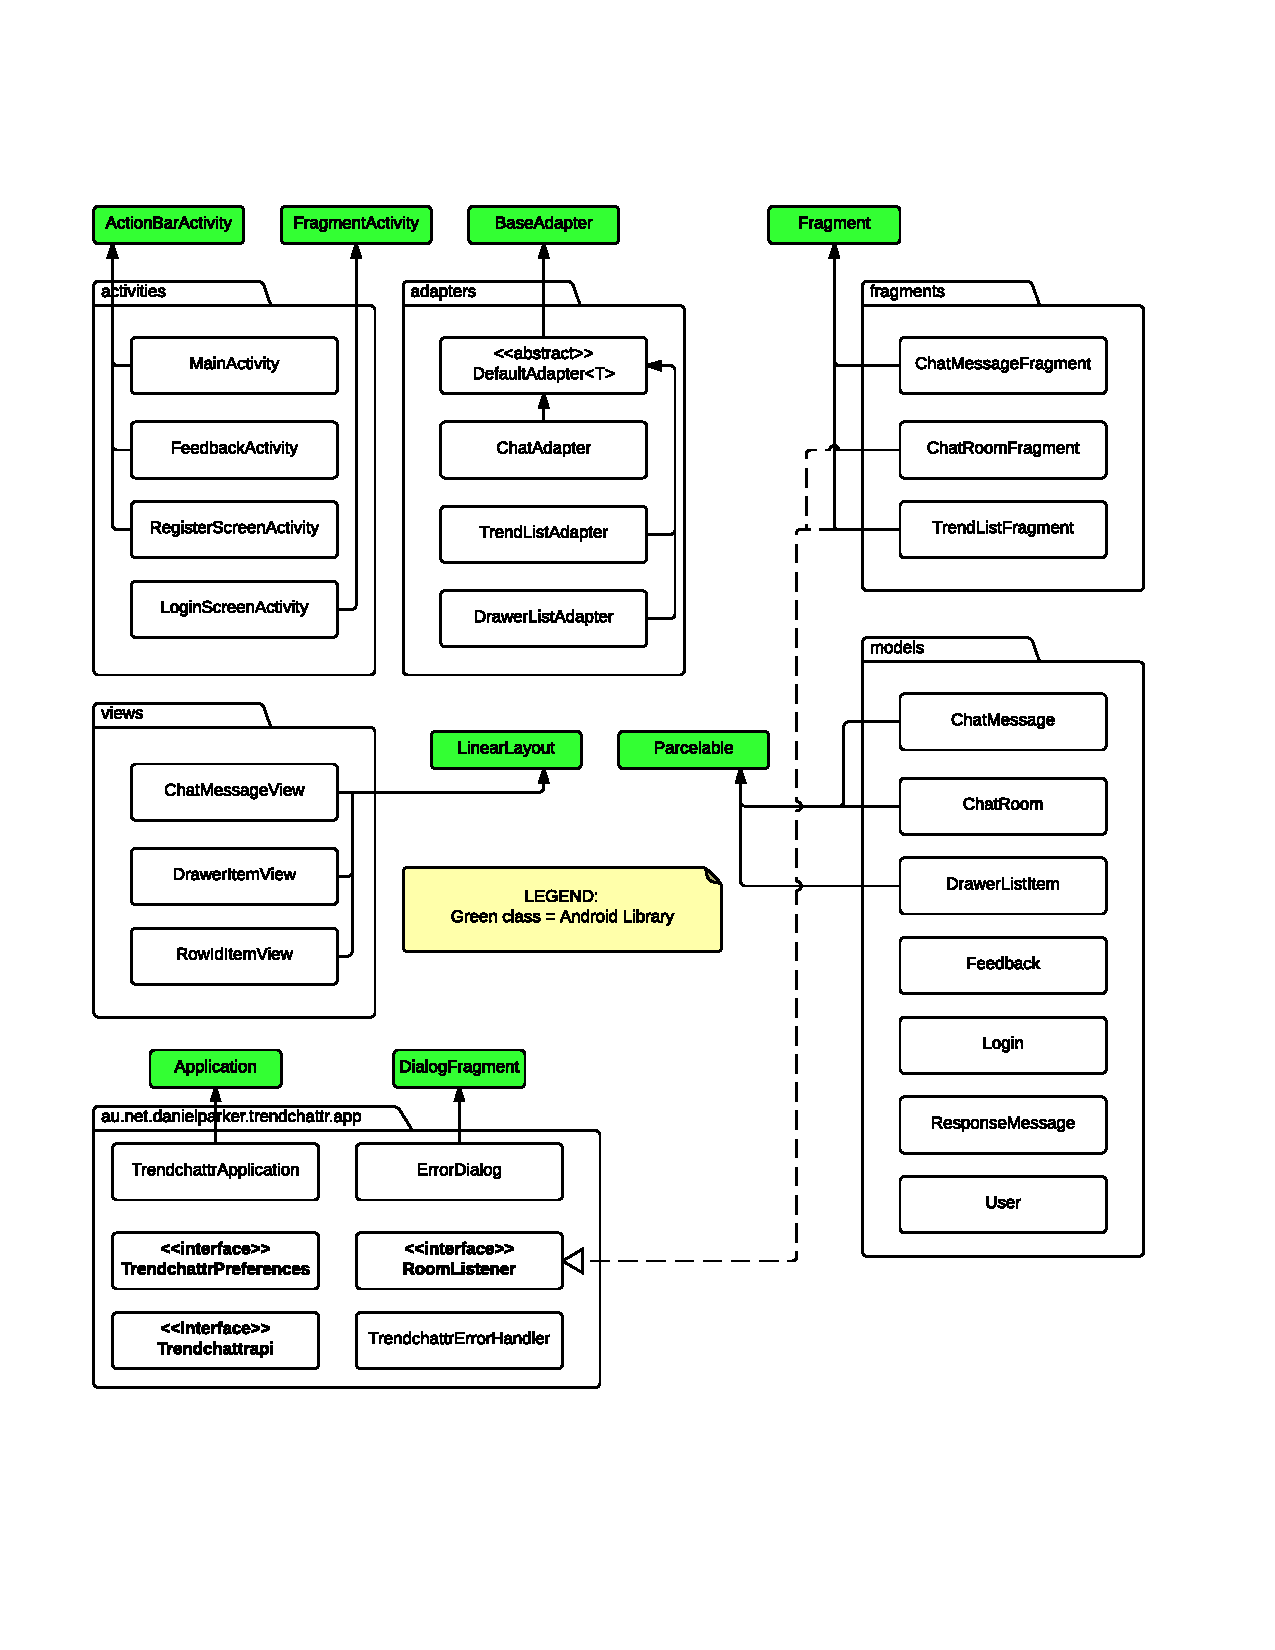
\includepdf[pages={1}]{classes.pdf}
  \subsection{Data Model}
  \begin{figure}[H]
    \centering{
      \fbox{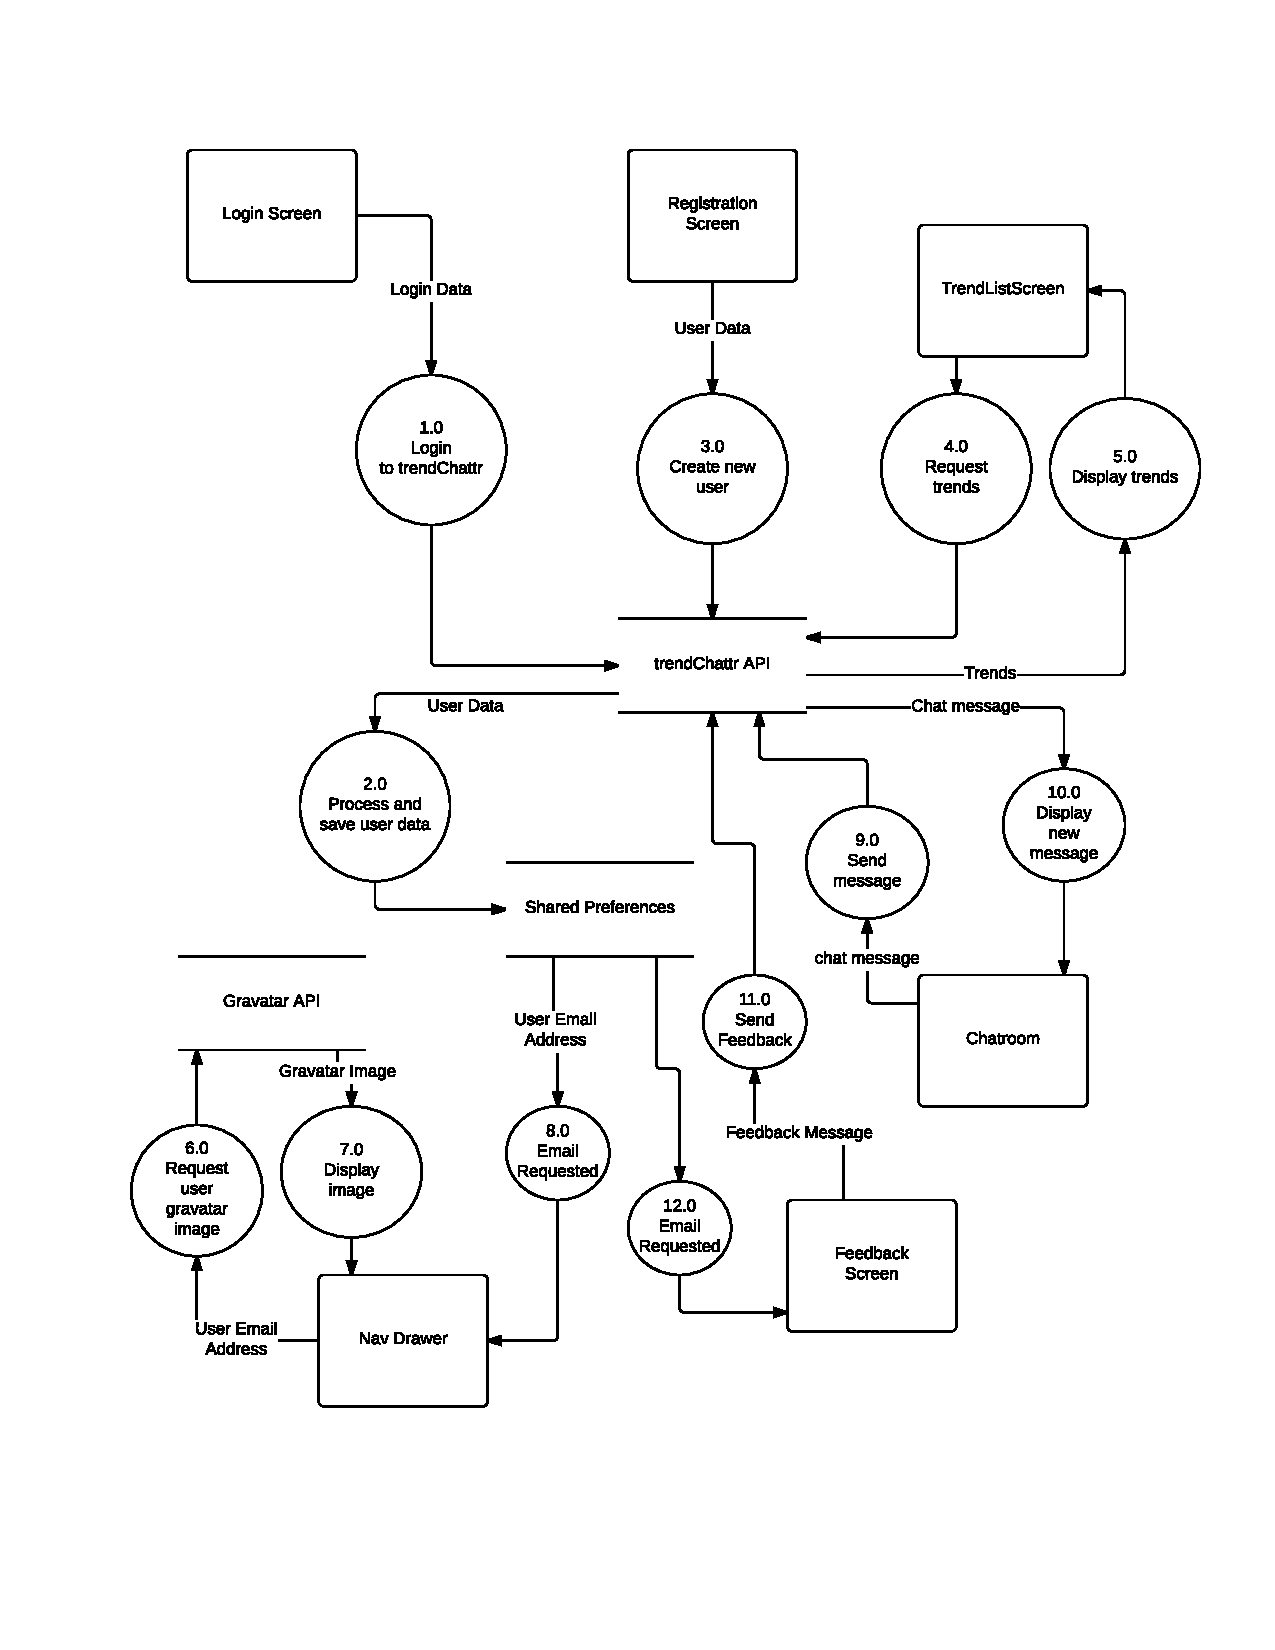
\includegraphics[width=\textwidth]{dataflow.pdf}}
    }
  \end{figure}
    %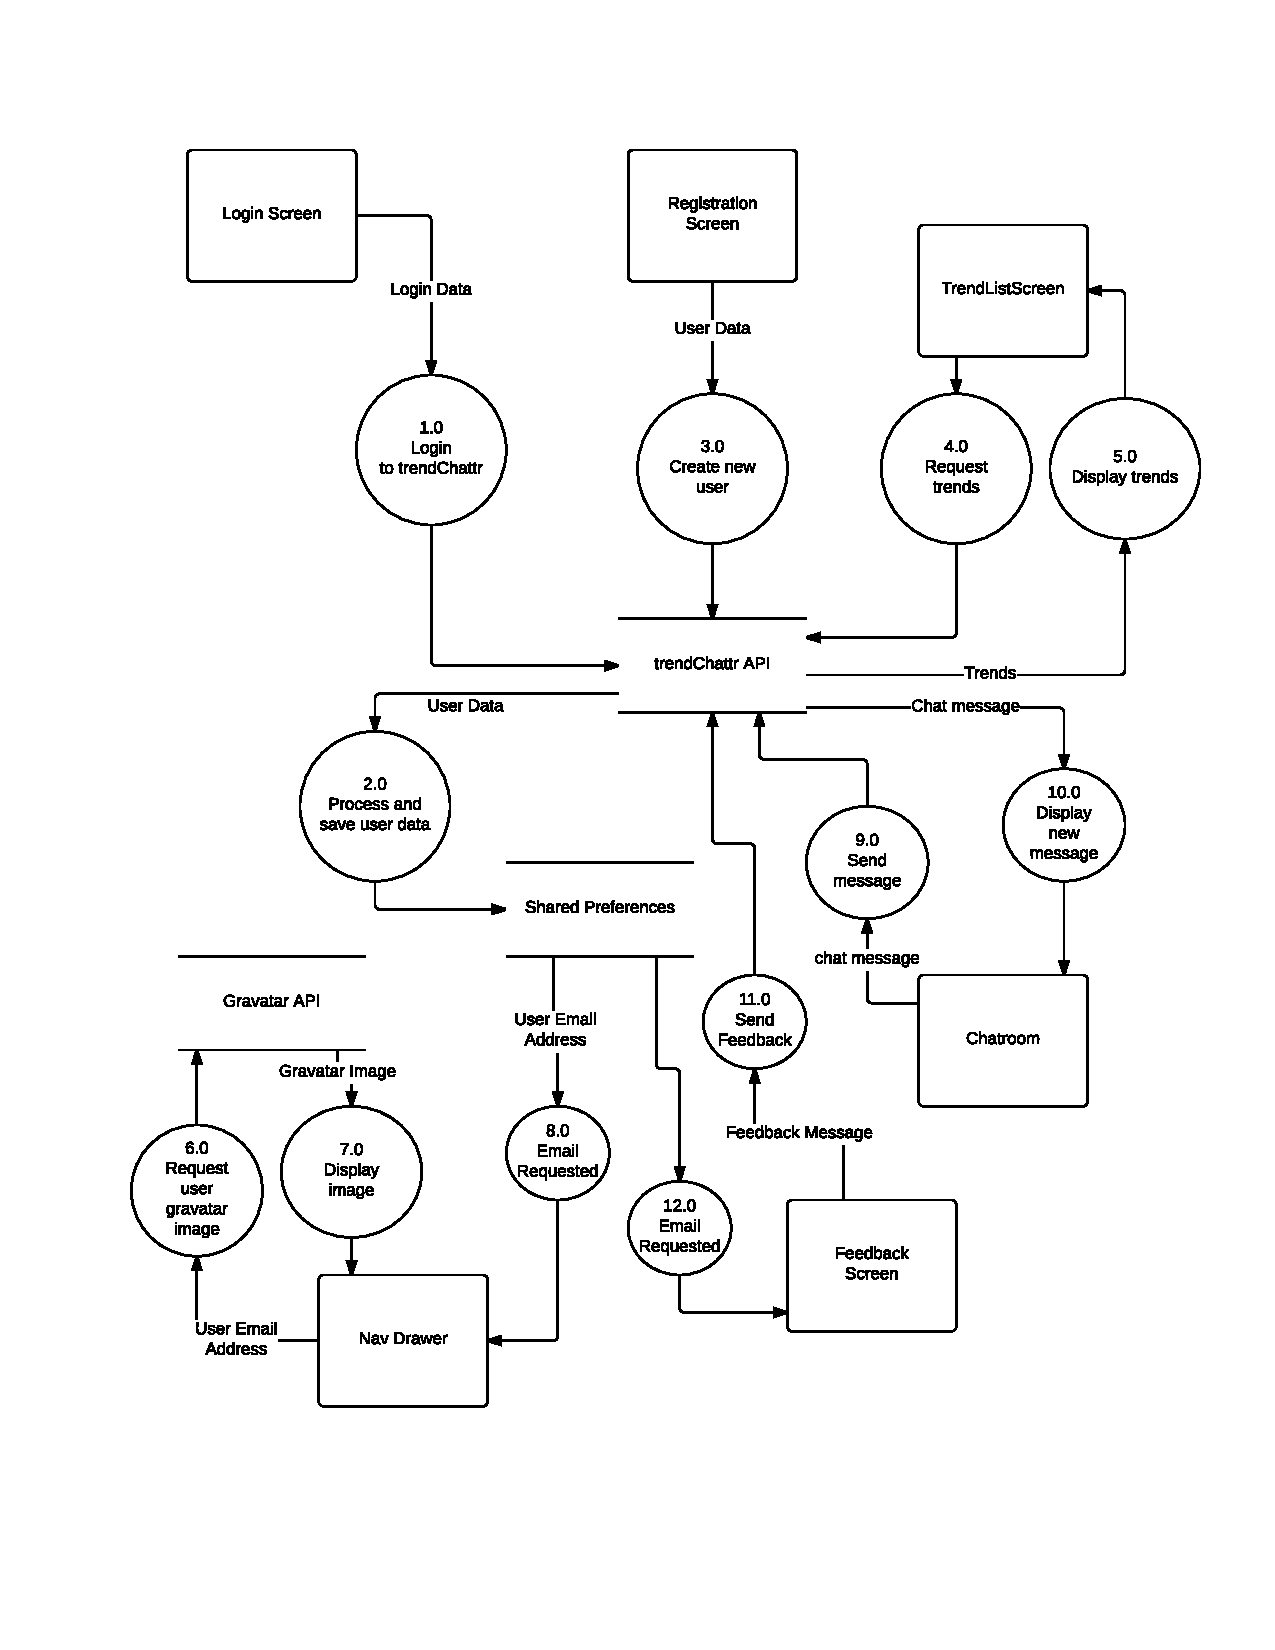
\includepdf[pages={1}]{dataflow.pdf}
\section{Visual Structure (Navigation)}
  \subsection{Navigation Flow Diagram}
    \begin{figure}[H]
      \centering{
        \fbox{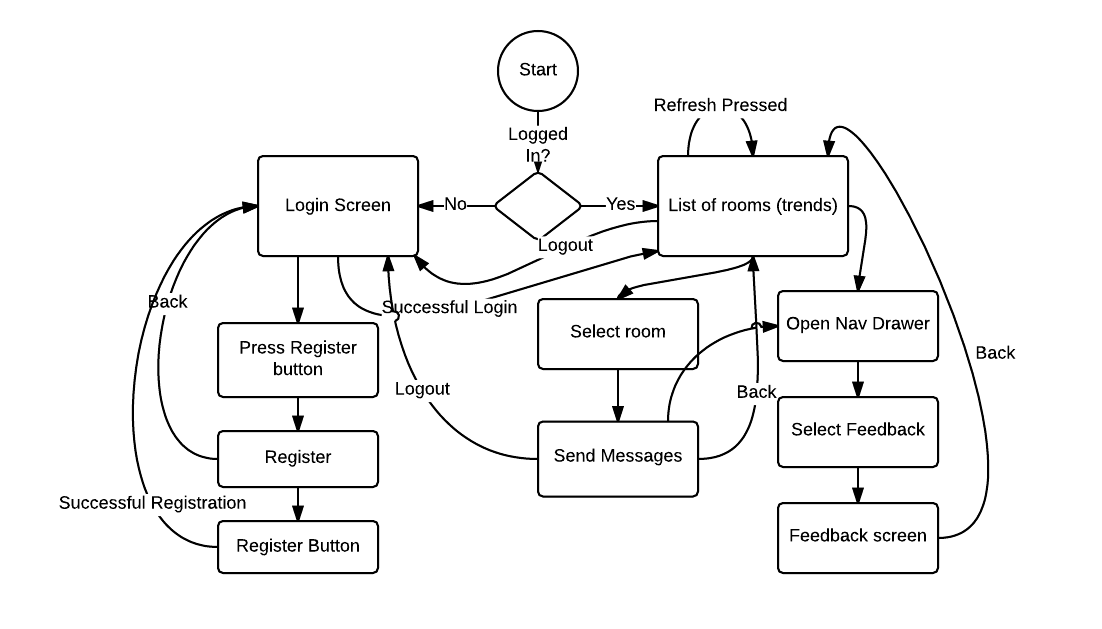
\includegraphics[width=\textwidth]{images/nav-flow.png}}
      }\\
    \end{figure}
\section{API Limitations}
  trendChattr utilises a few different library APIs, most supplied by the
  Android stack, and some third-party. The Android libraries while mostly stable
  and fully featured, do have the issue of compatibility. Unfortunately due to
  the requirement to have support back to API version 15, it was not possible to
  use the normal android libraries. Instead, the Android support libraries and
  appcompat libraries were used to allow for Material-like design and common
  navigation and visual functionality on devices running API 15+.

  This caused a variety of development setbacks as some of the Activities were
  written before realising this, and therefor required rewriting and sometimes
  complete restructuring to convert them to using the appcompat libraries. Some
  key areas which seem to be affected by this are, styling, action bars,
  navigation drawers, fragments and lists.

  The third-party libraries used include;
  \begin{itemize}
    \item{Retrofit}
    \item{Android Annotations}
    \item{socket.io-client}
    \item{cardview}
    \item{circularimageview}
    \item{jgravatar}
  \end{itemize}
  Most of these libraries are very stable and maintained which makes them very
  easy to work with. However socket.io-client and jgravatar do not seem to be
  heavily supported even though they do work out of the box. I would argue that
  in the case of jgravatar, the fact that it's not supported is of minor
  importance, as the library is trivial and due to it's open source license can
  be modified and maintained easily by me. In the case of socket.io-client it's
  not as simple as self-maintaining it and that is mostly due to the relative
  volatility of the socket.io server versions of which it needs to remain
  compatible with. The library is also a non-trivial program which could take
  quite a lot of time to learn. Both of these aspects combined with how crucial
  that library is to the chat feature in trendChattr makes it an issue to
  continue using.

\section{Retrospective and Considerations}
  So far I am very happy with the progress I have made and the speed in which
  I've made it in. This is partly because of the initial gains from using RAPPT
  to prototype the app, but also due to the relative ease of using the libraries
  that RAPPT uses, Retrofit and Android Annotations, as well as the availability
  of the jgravatar and socket.io-client libraries. I only had to modify the source
  of jgravatar to allow me to get gravatars larger than the 512px side width
  maximum enforced by the library.

  In general, I am happy with the structure of the app, though I would like to
  spend some time going back through each Activity and ensuring the consistent
  use of Android Annotations versus the manual procedure for certain tasks such
  as handling options menus. The source also lacks proper commenting and that
  is next on my list of things to go back and fix as I intend to continue
  developing this app with other developers.

  There are some things which I will need to consider in future versions of
  the app. I need to revisit whether socket.io is a good solution to the
  implementation of instant messenger chat, and whether there are
  solutions that will give better support to mobile devices, in that they
  integrate push notifications and chat history etc. I also want to spend time
  researching ways to effectively show chat messages from potentially hundreds
  or thousands of people in a single chat window. If this is possible and can
  be done nicely then it may revolutionise the way that we use chatrooms in
  the future. I am not convinced that the old IRC way of showing chat messages
  is the best way to do it, especially not for chatroom based conversations.
\section{Summary}
  In summary, the app has been designed mostly in line with the conventions
  and requirements of Android development in general, and also has had influence
  from the RAPPT generated prototype. Data-flow has been an interesting problem
  to solve with this app, and the solution that was found seems to work quite
  for the current usage levels. The experience has in general been very positive
  and has inspired me to continue developing this app and also an iOS and web
  application.
\section{References}
  \begin{enumerate}
    \item{
      ralfebert 2012, \textit{jgravatar}(v1.0.0)[Programming Library],
      viewed on 19 November 2014,
      \url{https://github.com/ralfebert/jgravatar}.
    }
    \item{
      Banes, C 2014, \textit{appcompat v21: material design for pre-Lollipop
      devices!}, Chris Banes, viewed 18 November 2014,
      \url{https://chris.banes.me/2014/10/17/appcompat-v21/}
    }
    \item{
      \textit{Creating a Navigation Drawer}, Developers, viewed 19 November 2014
      \url{https://developer.android.com/training/implementing-navigation/nav-drawer.html}
    }
    \item{
      Ricau, P 2013, \textit{Android Adapter Good Practices}, viewed 19 November
      2014, \url{http://www.piwai.info/android-adapter-good-practices/}
    }
  \end{enumerate}

\section{Appendix 1 (Planning and Design Document)}
  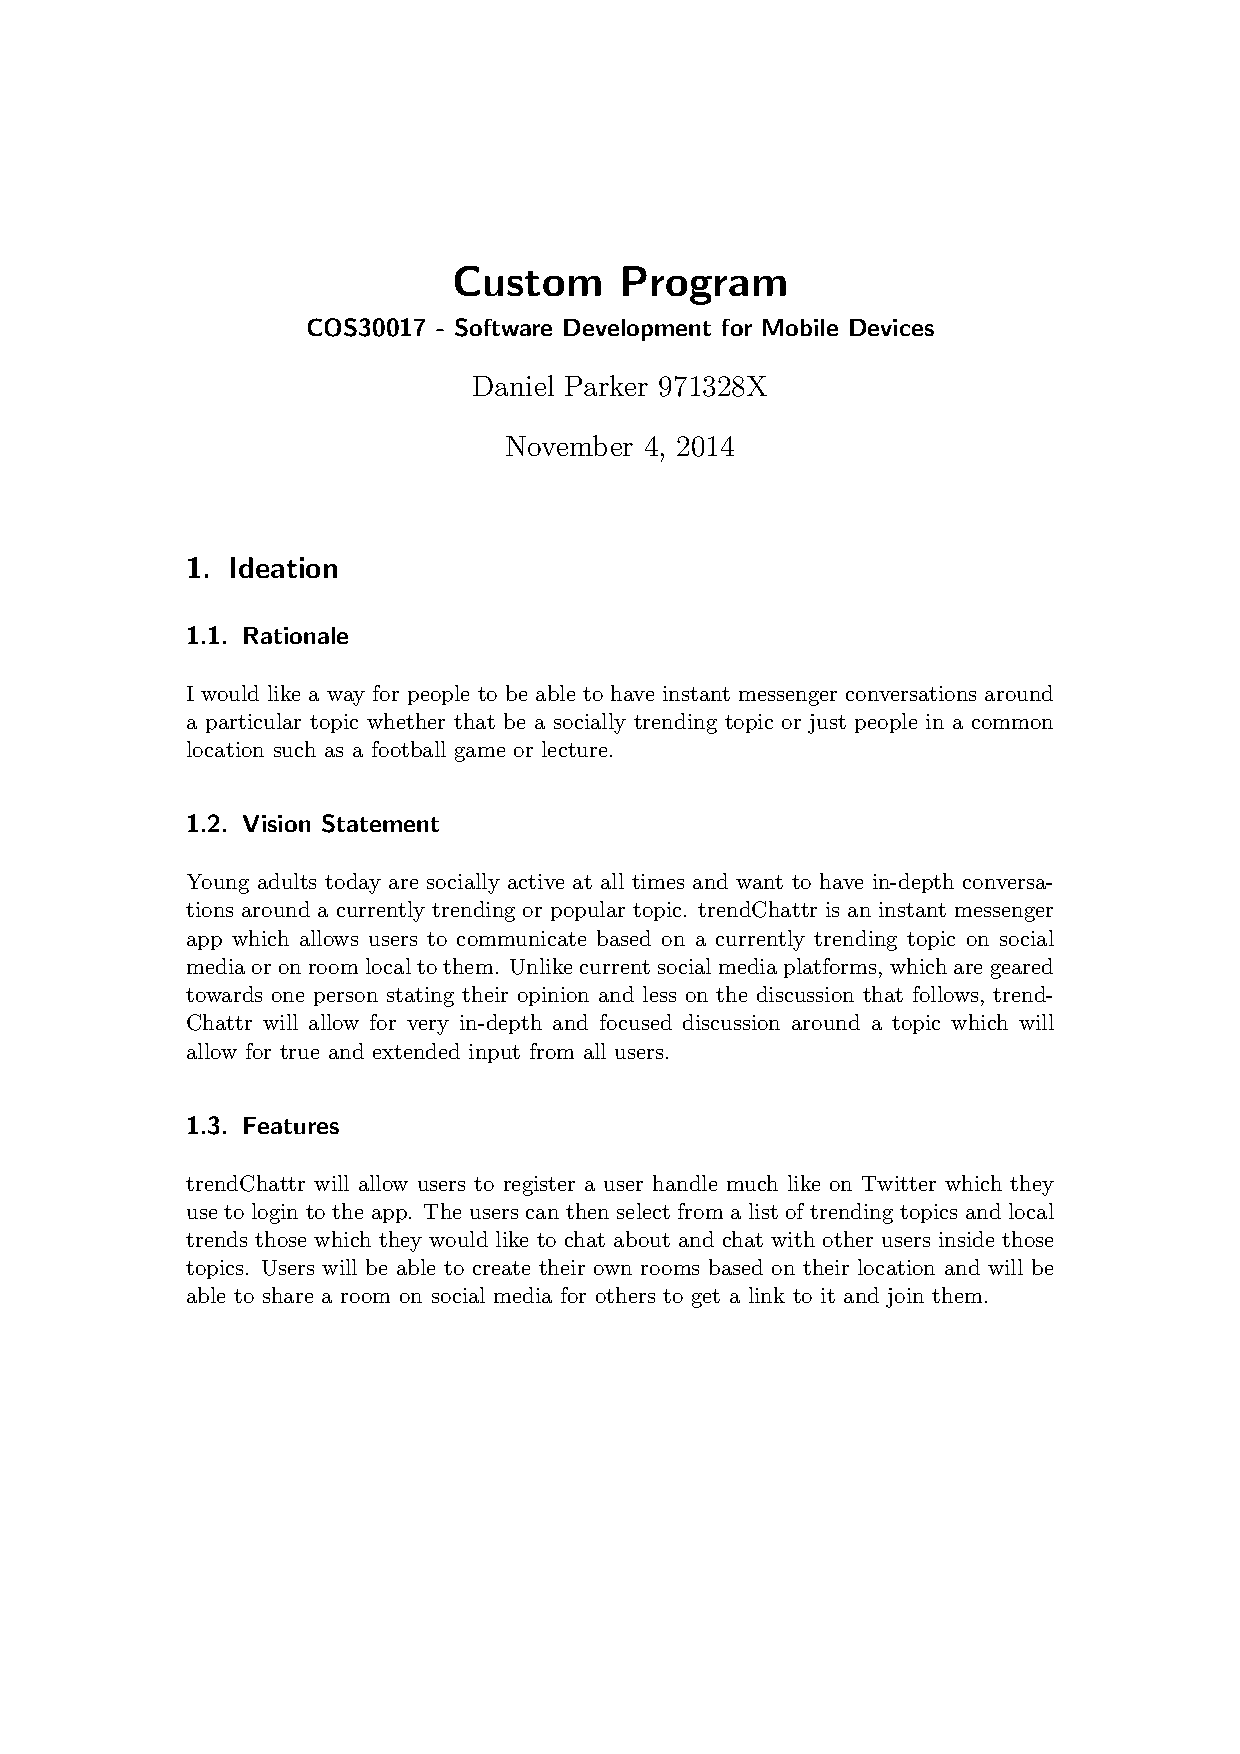
\includepdf[pages={1-6}]{design.pdf}
\section{Appendix 2 (App Screenshots)}
  \begin{figure}[H]
    \centering
    \begin{subfigure}{.5\textwidth}
      \centering
      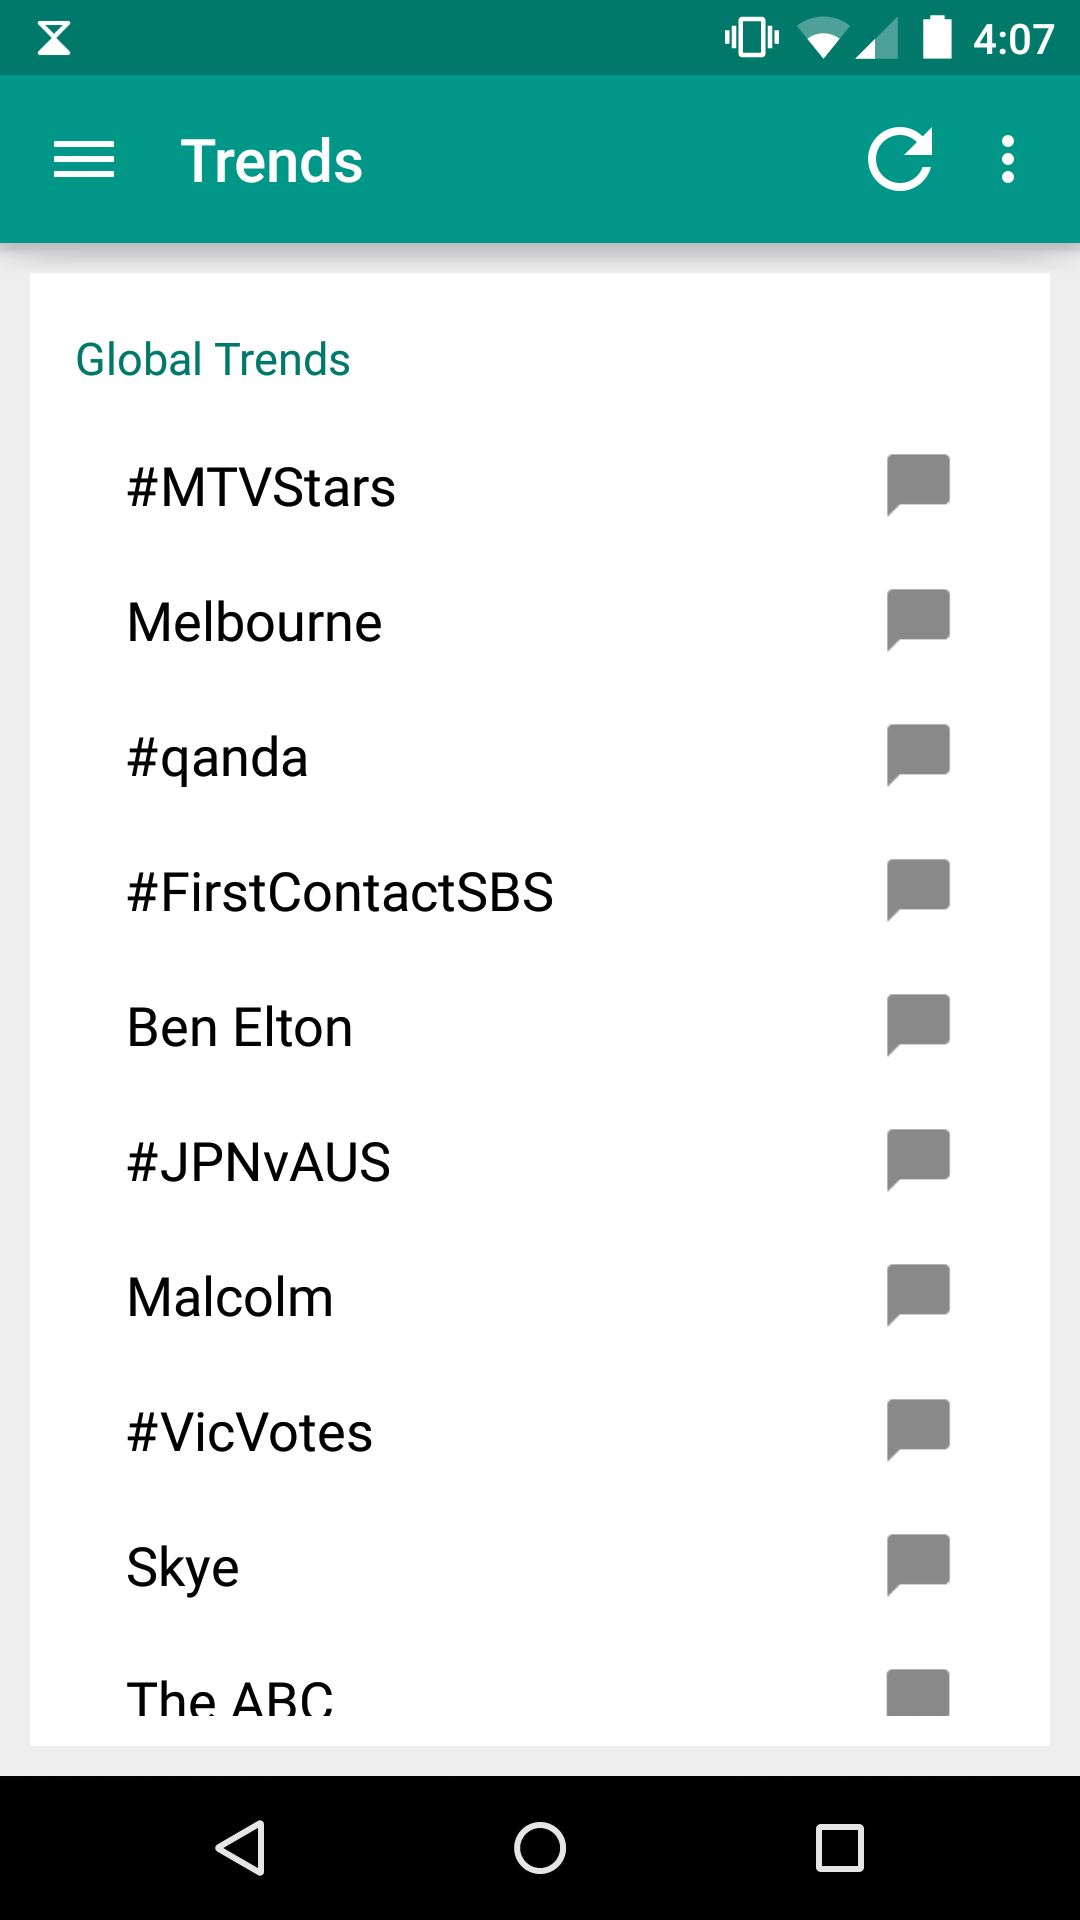
\includegraphics[width=.7\linewidth]{images/ss1.png}
    \end{subfigure}%
    \begin{subfigure}{.5\textwidth}
      \centering
      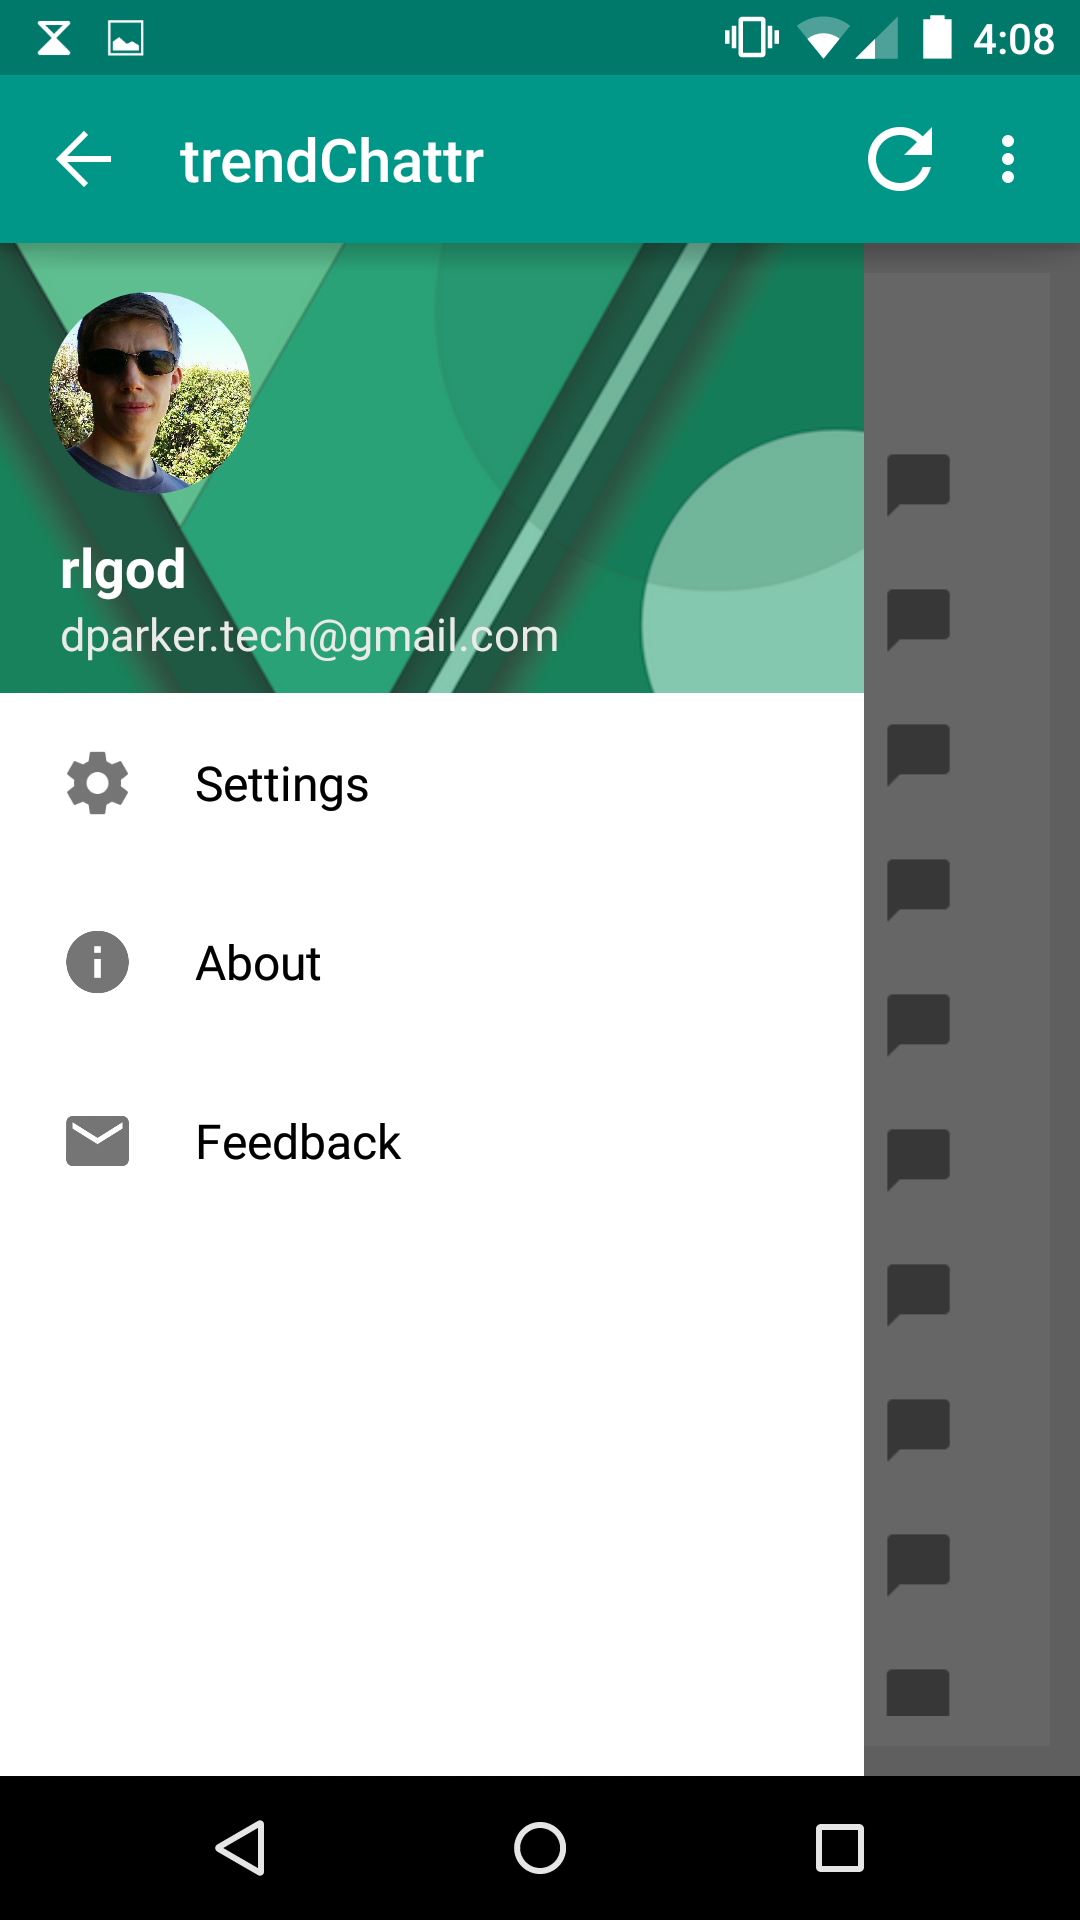
\includegraphics[width=.7\linewidth]{images/ss2.png}
    \end{subfigure}
  \end{figure}

  \begin{figure}[H]
    \centering
    \begin{subfigure}{.5\textwidth}
      \centering
      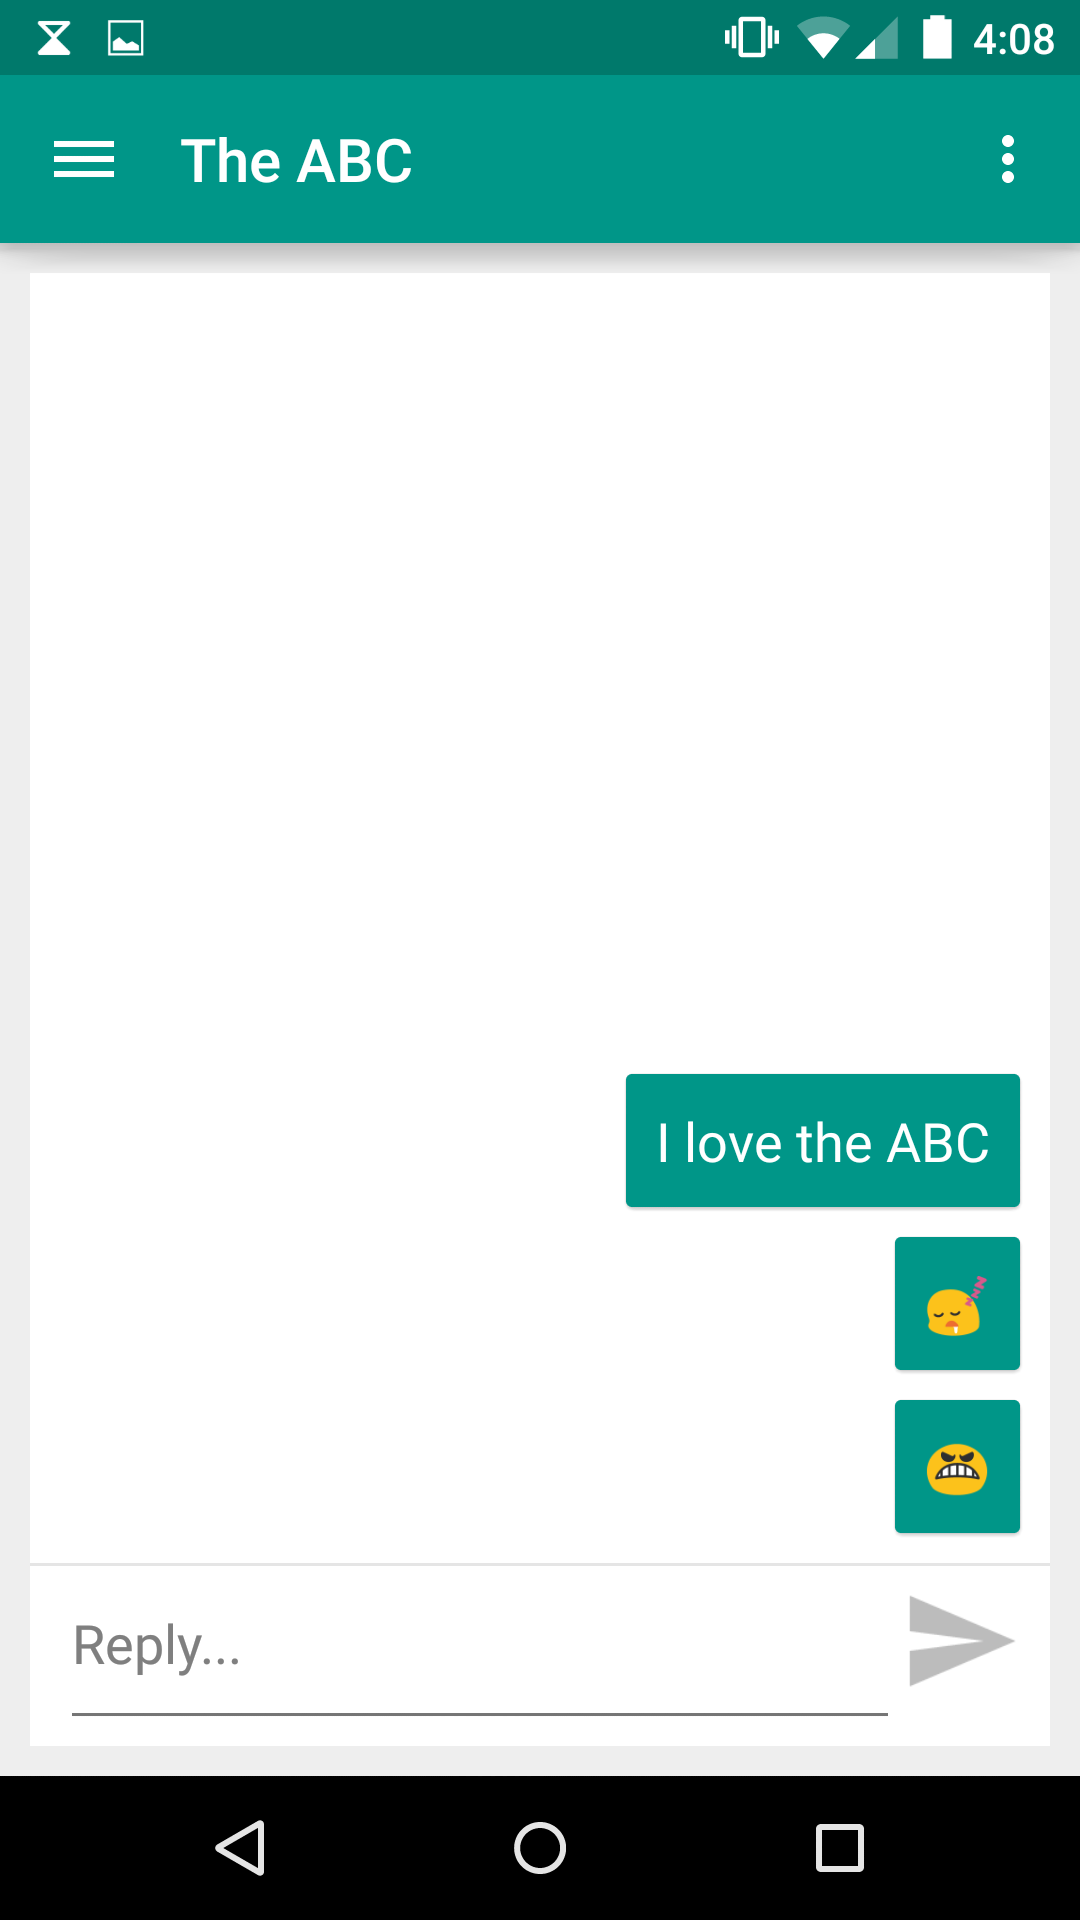
\includegraphics[width=.7\linewidth]{images/ss3.png}
    \end{subfigure}%
    \begin{subfigure}{.5\textwidth}
      \centering
      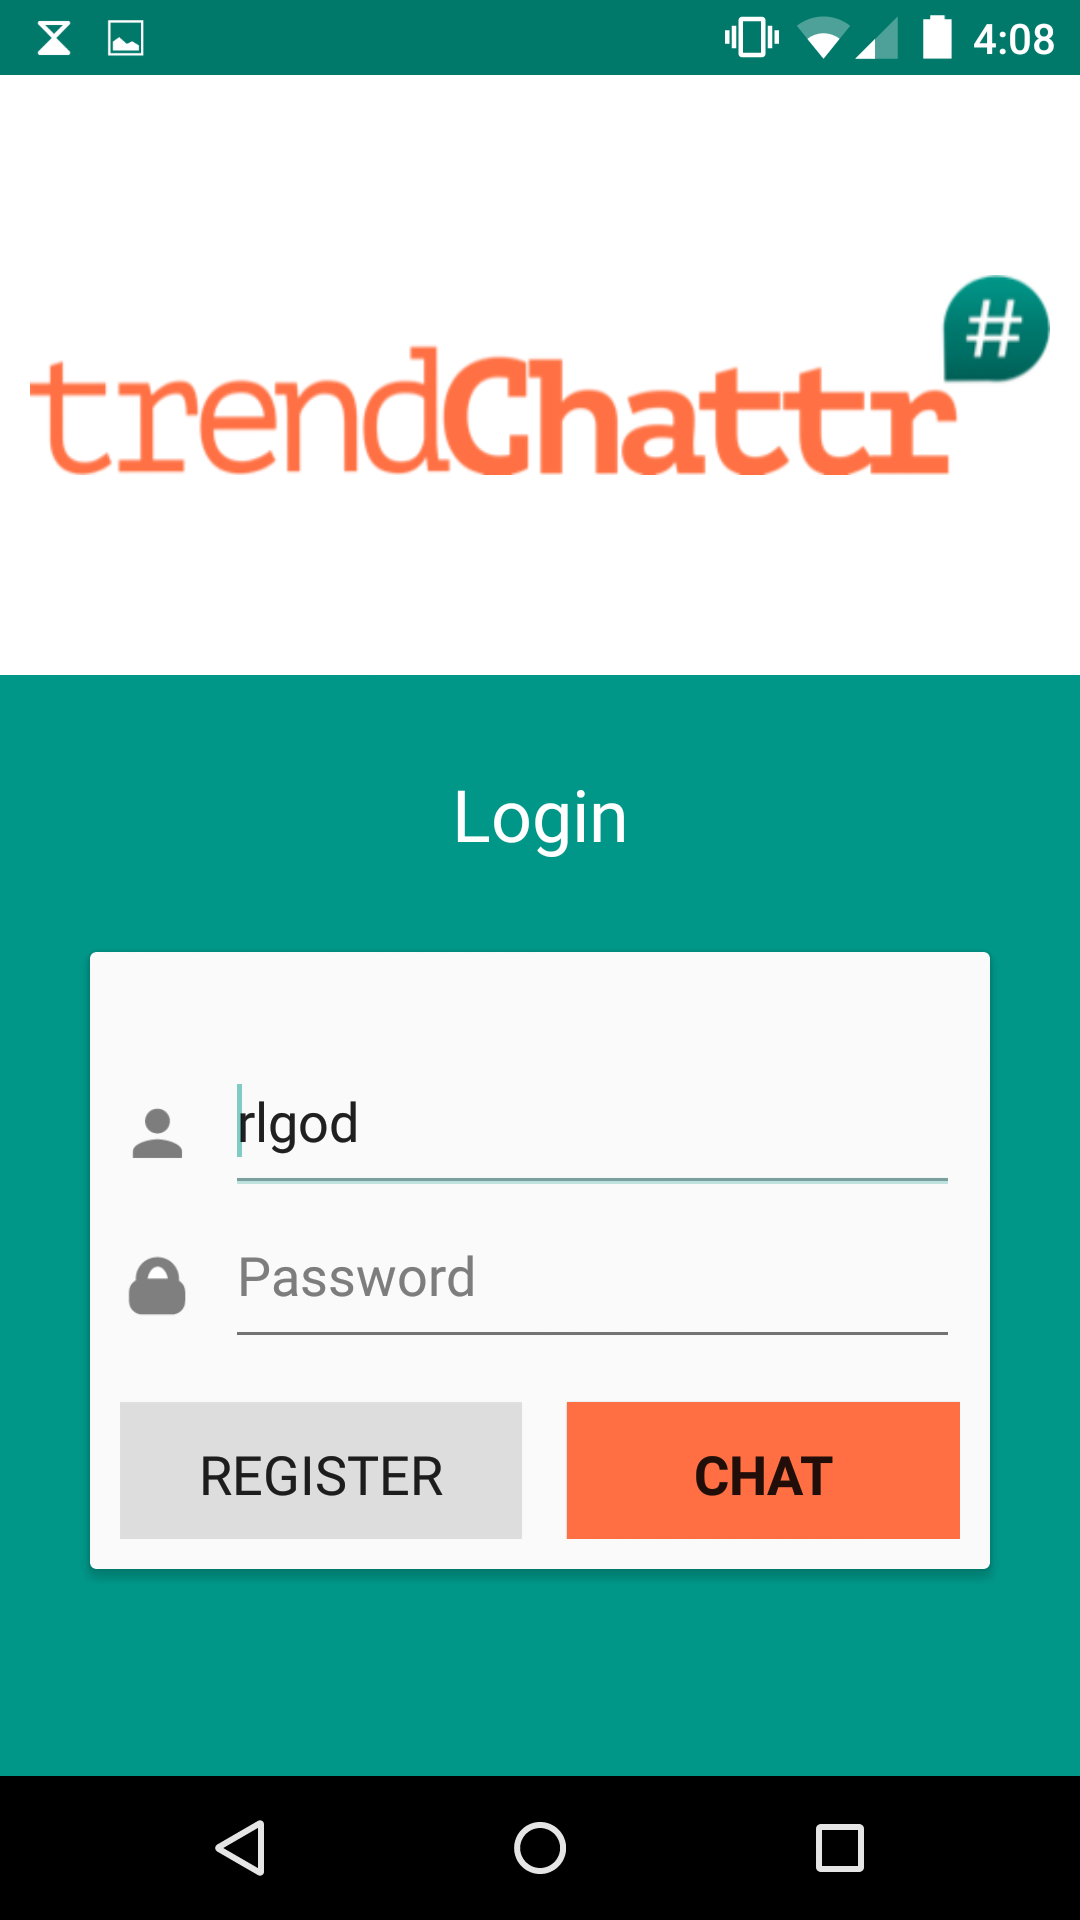
\includegraphics[width=.7\linewidth]{images/ss4.png}
    \end{subfigure}
  \end{figure}

  \begin{figure}[H]
    \centering
    \begin{subfigure}{.5\textwidth}
      \centering
      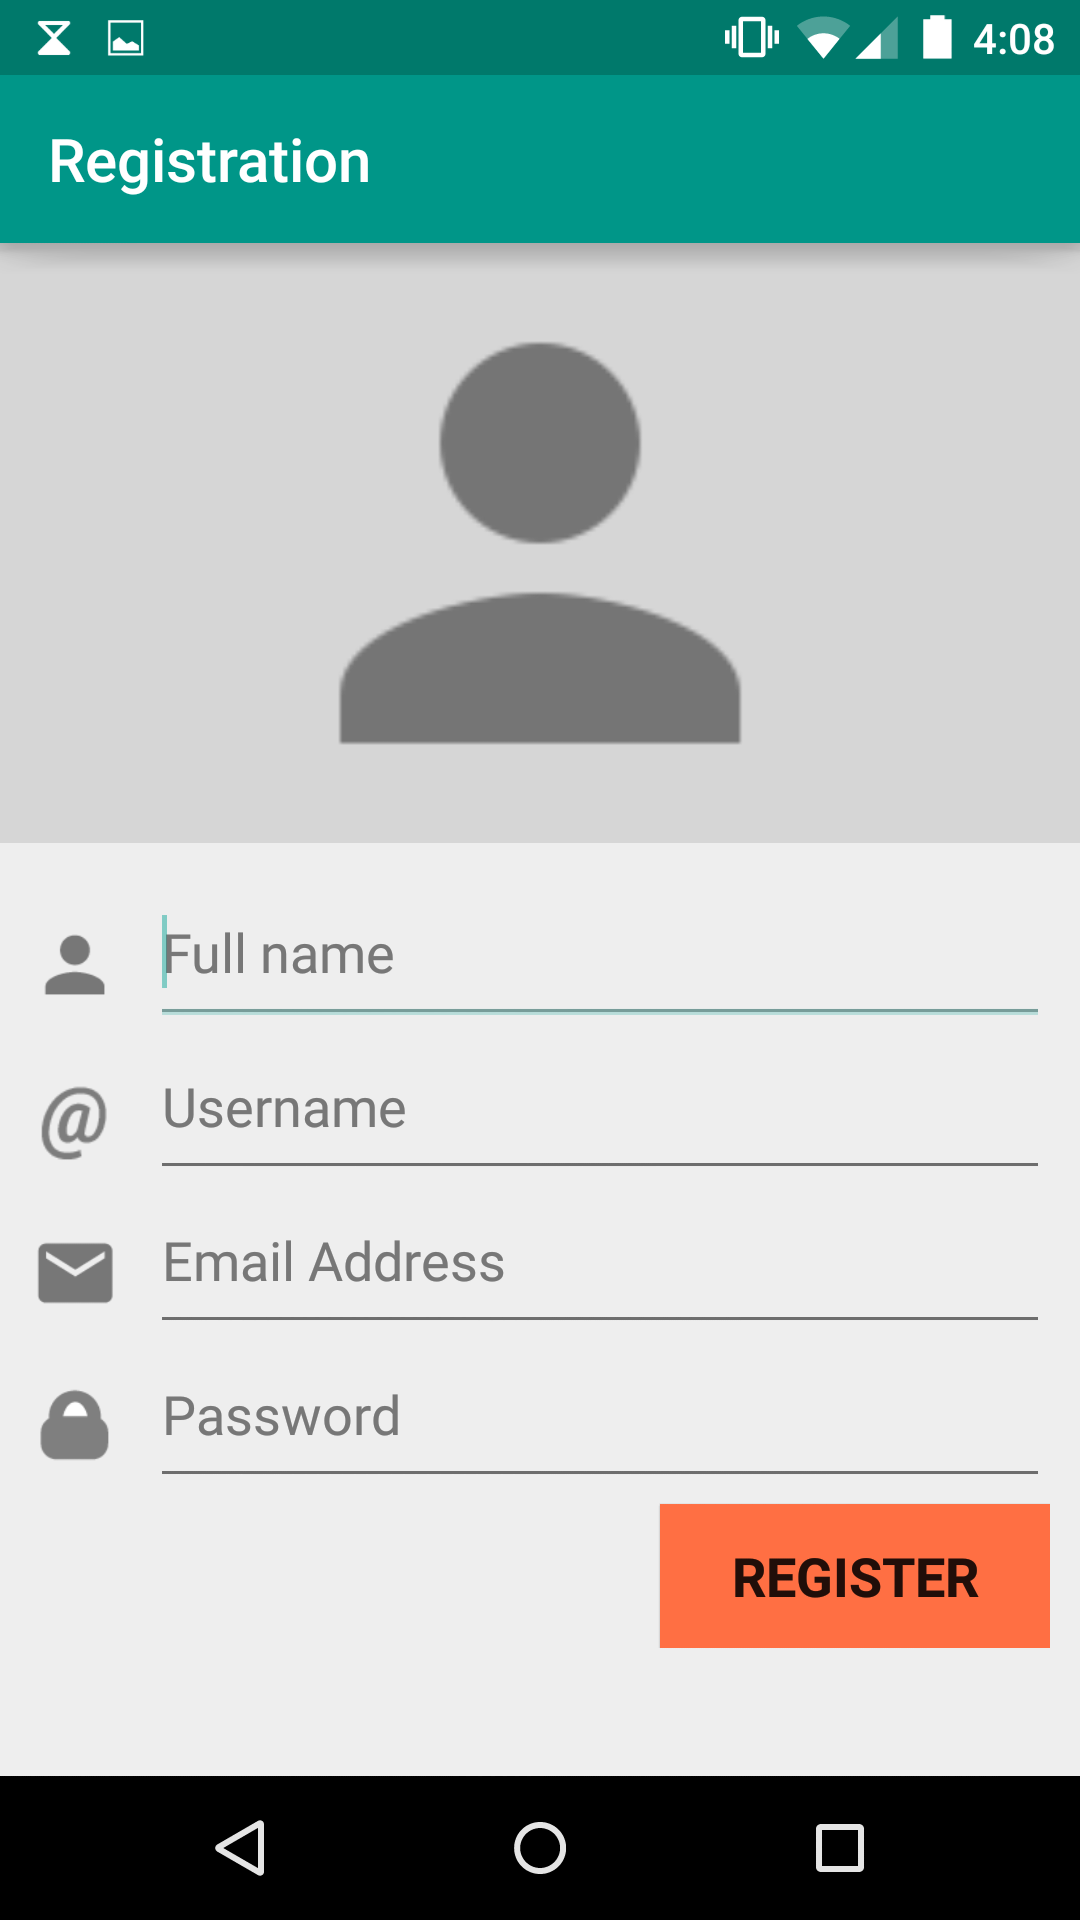
\includegraphics[width=.7\linewidth]{images/ss5.png}
    \end{subfigure}%
    \begin{subfigure}{.5\textwidth}
      \centering
      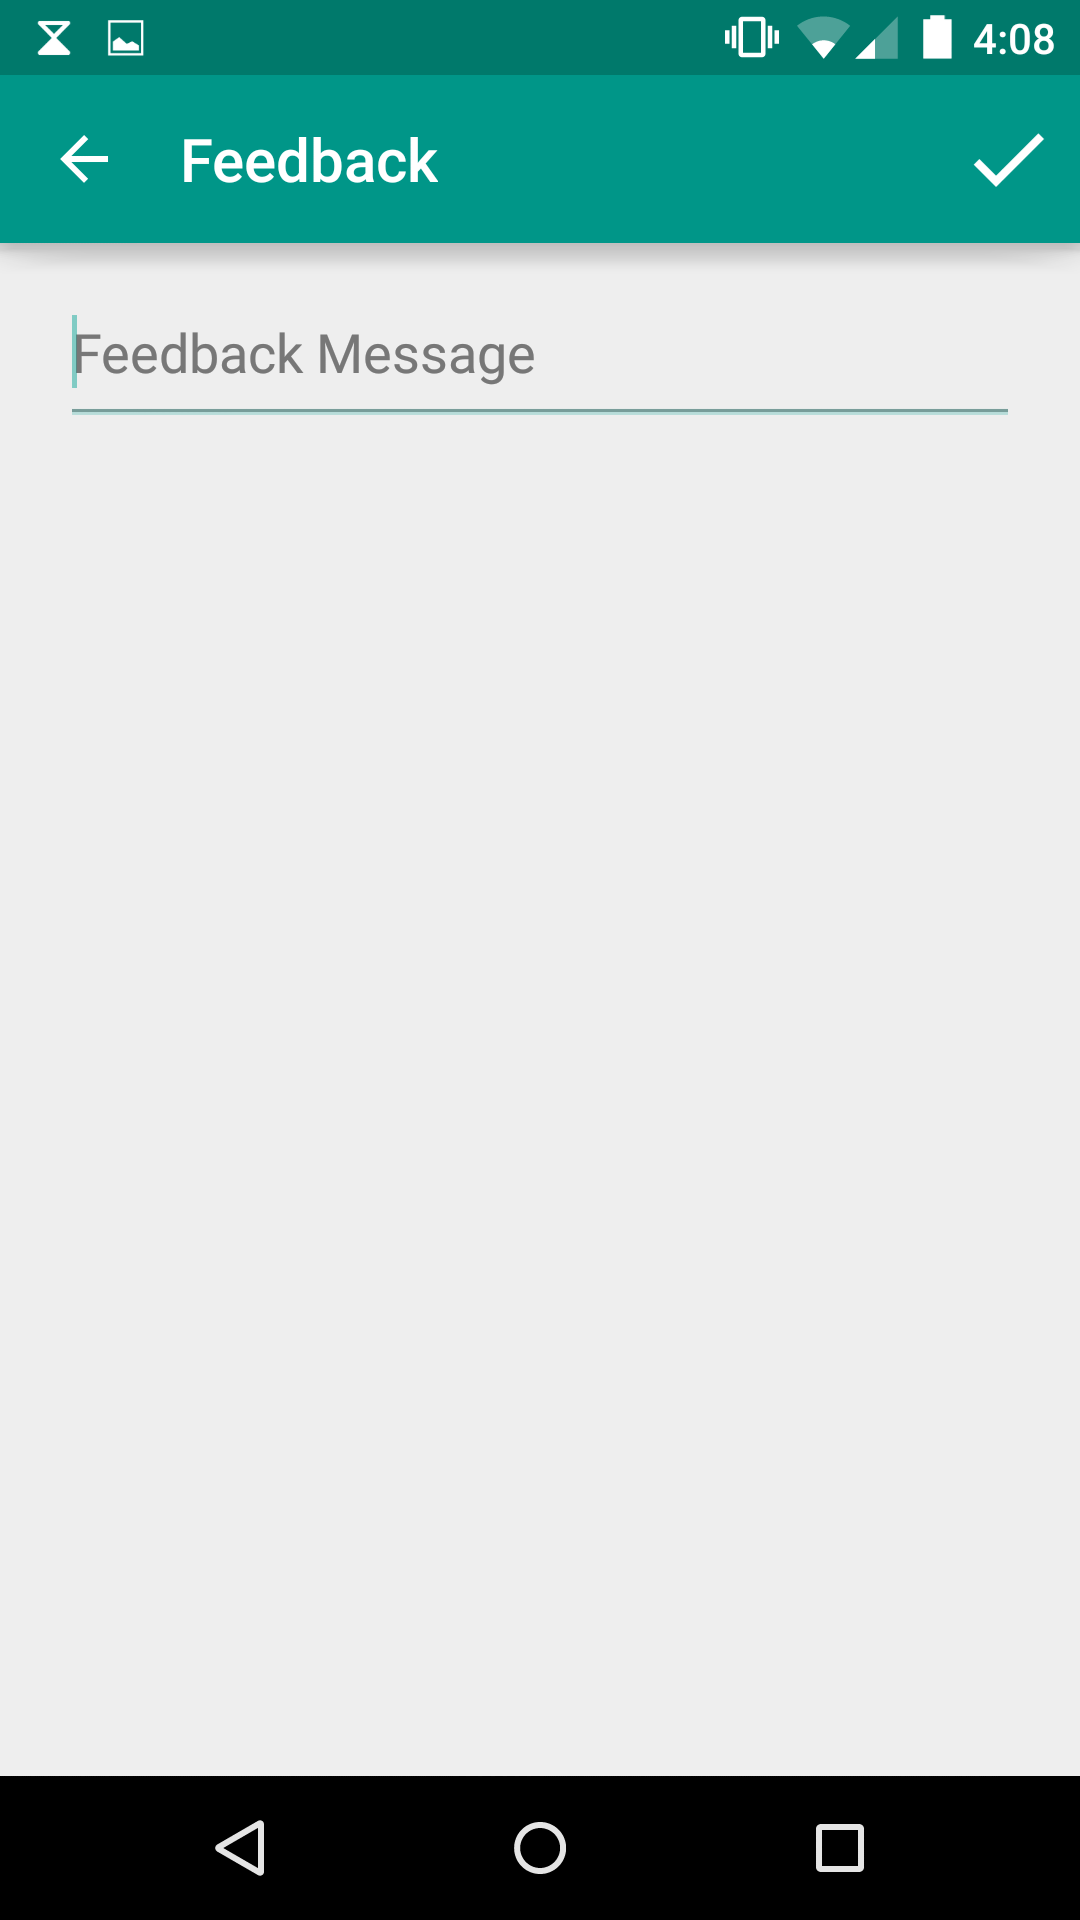
\includegraphics[width=.7\linewidth]{images/ss6.png}
    \end{subfigure}
  \end{figure}
  % \begin{figure}[H]
  %   %\centering{
  %     \fbox{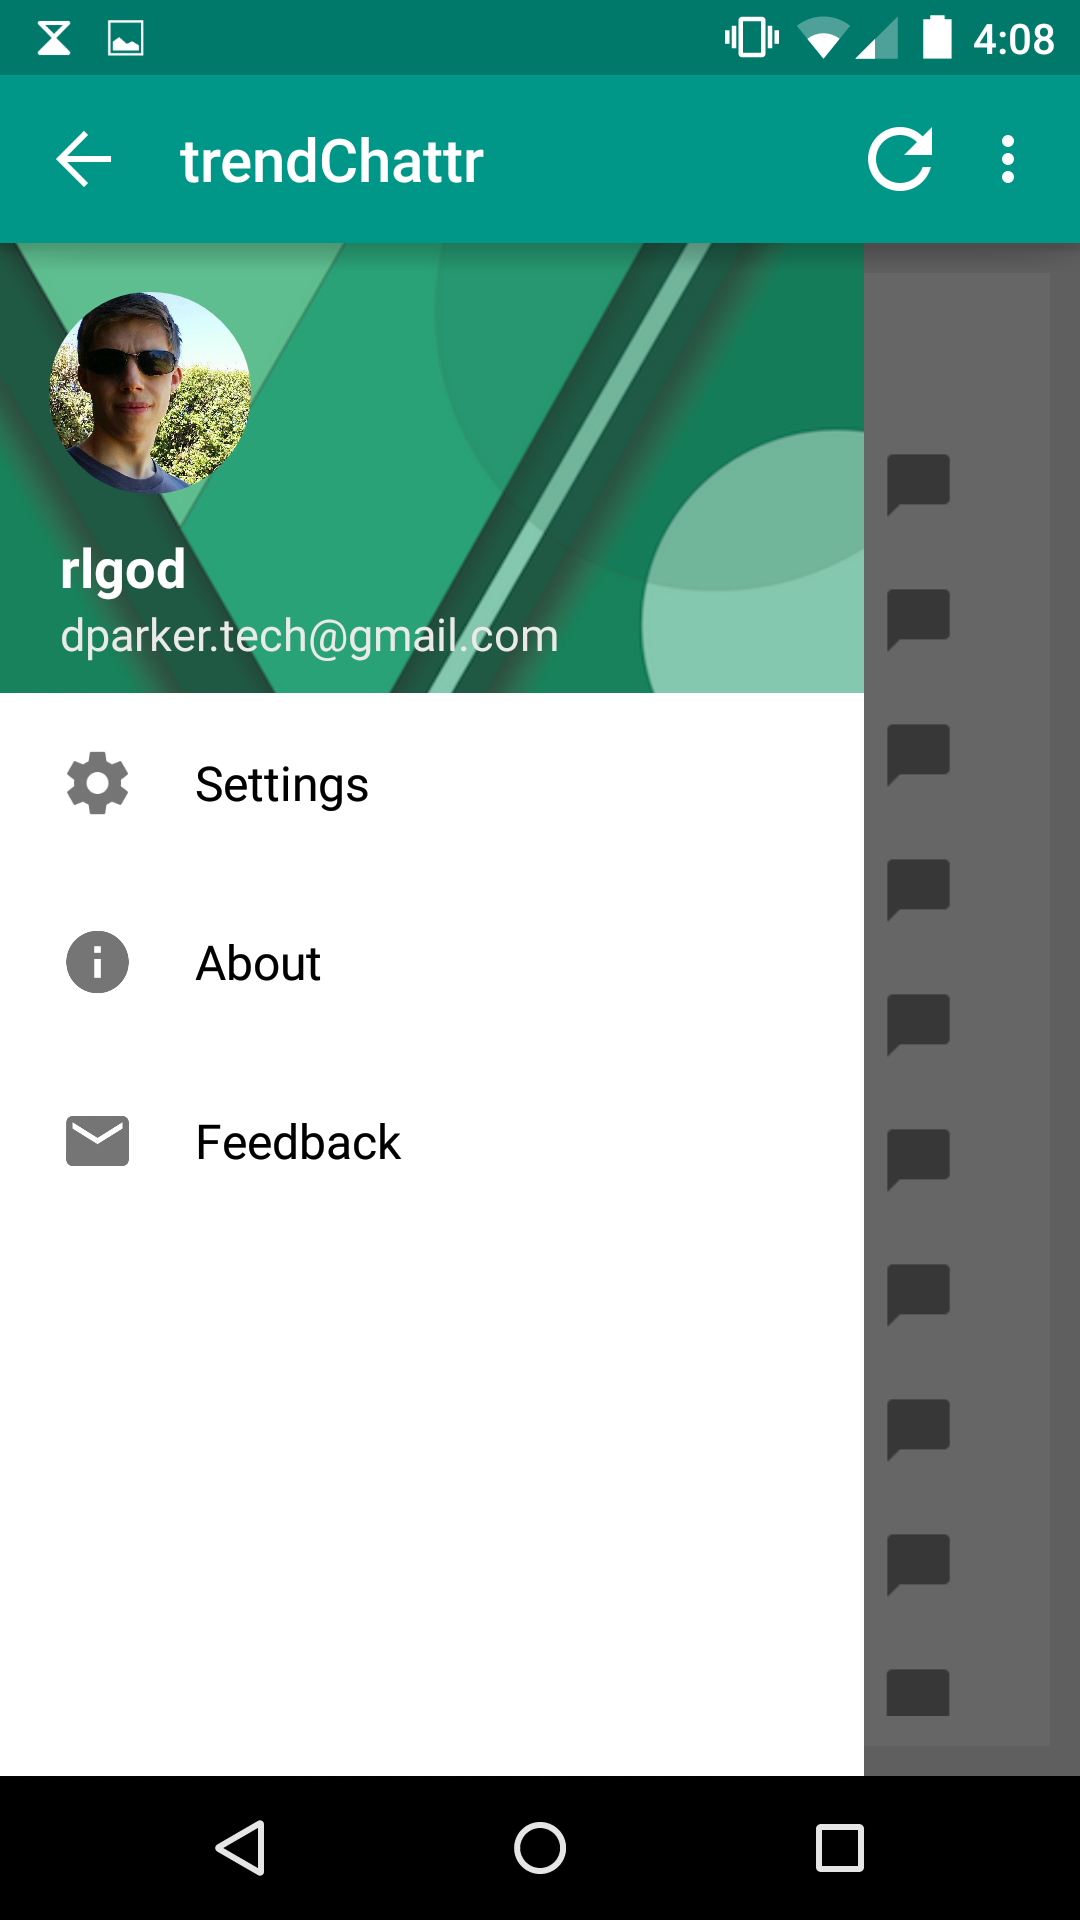
\includegraphics[width=6cm]{images/ss2.png}}
  %   %}\\
  % \end{figure}

\end{document}
